\chapter{Multi-domain data} \label{chap:data}

Although there is a need for multi-domain semantic similarity measures in the generality of the semantic web community, specifically within the scientific community, there is still a lack of substantial data this technique can be applied to. This, it can be argued, seems a contradictory state of affairs. Either there is data and as such the techniques to analyse them are needed, or there is a lack of data and the techniques are superfluous.

The truth is that semantic similarity is not a \emph{pressing} need for state-of-the-art semantic web practices, nor is it fundamental to \emph{current} scientific progress. In generic areas of the semantic web (outside the biomedical scope), ontologies are not even highly used, and knowledge is not \emph{well} represented, by which I mean
\begin{paralist}
    \item that ontologies are not consistent, either internally or with the external world;
    \item that the represented knowledge is severely incomplete; or
    \item that there is no way to integrate that knowledge with other ontologies, since the principles of interoperability are overlooked or neglected.
\end{paralist}
For example, \texttt{dbpedia.org}~\citep{Bizer2009a} is a collection of information spanning most domains of knowledge (based on the structured information of Wikipedia), but it is particularly rich in instance-level properties, not in ontological knowledge: while it contains the information that ``Lisbon'' \prop{has-timezone} ``Western European Time'', there is no representation of geospatial knowledge, which would, in particular, contain the axiom that \prop{has-timezone} is a property that can be applied to instances of \term{Place} and whose value must be a \term{Timezone}. Nevertheless, there is a small number of ontological information expressed in OWL, such as ``\term{Capital} \prop{is-a} \term{City}''.\looseness=-1

In contrast, while some areas of research, particularly in biomedical domains, are developing an increasing number of ontologies, there is still a lack of data annotated with them. One notable exception is the Gene Ontology, which is extensively used to annotate proteins and the results of genomic experiments (see \secref{sec:concepts/semantic-annotation} and \chpref{chap:validation}). This exception suggests that the lack of data does not correspond to a fundamental characteristic of scientific knowledge; instead, I argue that there is no motivation to annotate in the first place because there are not many tools able to explore the data. Once these tools start to appear, more data will be emerge. In light of this, one of the tasks I executed was multi-domain semantic annotation acquisition. These data allow the application of similarity measures on real datasets.

In this section, I present three datasets that were collected for exploiting semantic similarity, in three different areas of research: epidemiology, metabolism, and computational modelling of biological processes. For a list of the ontologies used by these datasets, see \appref{app:ontologies}.


\section{Epidemiology Dataset} \label{sec:data/epiwork}

Epidemiology is inherently a multidisciplinary subject, relying on areas of knowledge as diverse as medicine, biology, statistics, sociology and geography~\citep{Porta2008}. Even under the scope of medicine and biology, epidemiology deals with chemical compounds, diseases, symptoms, environmental conditions, methods of transmission, vaccines, \etc.

Given this multitude of domains, processing, storing and preserving epidemiological data is not straightforward. To explore ways of managing this type of data, a consortium of several partners established the Epiwork project, aimed at developing the appropriate framework of tools and knowledge to design epidemic forecast infrastructures, including an epidemiology data repository that was developed by the LaSIGE partner (see \secref{sec:auxiliary-projects/epiwork} for a summary of my contributions to the Epiwork project).

One of the most important functions of a data repository is the ability to search within its resources. A search box that can be used to convert a user query into a list of results is essential for the widespread adoption of the repository. There are at least two possible ways to implement this feature:
\begin{paralist}
    \item allow free text searches that try to map the words in the query to the words in the content of each resource; or
    \item annotate the resources of the repository with metadata that reflect its content and use the query to search within these metadata.
\end{paralist}
While the first way maps roughly to how web search engines work today, the second way is much more aligned with the idea behind the semantic web, with all its advantages (see \secref{sec:concepts/semantic-annotation,sec:concepts/semantic-web}) and, as such, the team behind the Epidemic Marketplace decided to provide a way for users and curators to annotate their resources.

Given the multidisciplinary nature of epidemiology and the resources contained in the Epidemic Marketplace, a multi-domain semantic similarity measure would be an asset to assist the search functionality, which would require a means to compare resources based not on one domain in particular (\eg diseases), but on all the domains of annotation.

Consider a user searching for resources about ``infectious diseases''. Using the Human Disease Ontology (\ontology{DOID}), specifically its class-subclass hierarchy, the search functionality can successfully retrieve all resources with data on \term{Flu}, \term{AIDS} and other infectious diseases. However, it can happen that the user queries for very specific resources (for example by over-specifying the disease, the symptom or the location of an outbreak), resulting in an empty list of retrieved resources. In such cases, it is possible to find some results that \emph{almost} satisfy the query by comparing the repository resources with the query. For example, the query ``2009~European infectious disease outbreaks that manifest through coughing'' could be satisfied with a resource about a 2010~European infectious disease outbreak that manifested through sneezing. Additionally, when the query does return some results, semantic similarity can be used to sort those results according to how related they are to the original query.

On the other hand, semantic similarity provides a mechanism to implement a ``Related resources'' section in the repository. Users looking at the contents of a particular resource are usually interested not on a single resource but on a collection of them, all of which are related. For example, a user looking at a resource that contains data about flu-like diseases is probably also interested in resources about other infectious pulmonary diseases. Having a section of the web page dedicated to these related resources removes the need for the user to make complex and sometimes unintuitive queries to the search feature.

One of my contributions to this project was the development of a semantic metadata model and a Network of Epidemiology-Related Ontologies (NERO). Both are used to assist the annotation of epidemiological resources: the metadata model describes the type of information that a resource needs and NERO provides concepts for the annotation (see \secref{sec:auxiliary-projects/epiwork}).

During the Epiwork project, it was possible to annotate a set of $228$~resources, each one containing a reference to an open-access paper from an epidemiology journal (the annotation process itself was conducted by someone else in the project, not me). Each of these resources is annotated with a set of concepts from NERO according to the semantic metadata. Hence, this dataset contains metadata on domains such as ``environment'', ``diseases'', ``symptoms'', ``modes of transmission'', ``demography'' \etc.

By leveraging on NERO to represent the concepts that each paper refers to, the papers become enriched with semantic information and can, therefore, be used in semantic analysis. While there is no explicit quantitative assessment of similarity or relatedness between these resources, and as such there is still no gold-standard that can be explored in the development of multi-domain semantic similarity, doing so is not beyond the realm of possibilities, since the resources are already annotated. As such, I gathered this dataset to run semantic similarity on it, as we will see later in \chpref{chap:multidomain}.

A summary of the relevant annotations for these resources is given in \tabref{tab:epiwork-summary}. In this table, I make use of three statistics that depict the annotation panorama of these resources with respect to a single domain:
\begin{description}
    \item[Coverage] This is the fraction of resources that have at least one annotation in the domain.
    \item[Volume] This is the average number of concepts from this domain in the resources. It is calculated with respect to the resources that have at least one annotation, which means that the minimum value is~$1.0$.
    \item[Diversity] This is the number of distinct concepts from the domain that are used throughout all the dataset.
\end{description}

\begin{table}
\caption[Summary of the annotation in the epidemiology dataset]{This dataset corresponds to $228$~epidemiology resources extracted from the Epidemic Marketplace. The first two columns describe the domains and ontologies used to annotate the resources. The rest of the columns provide statistics for each domain. A description of each statistic is given in the text.}
\label{tab:epiwork-summary}
\centering
\small
\begin{tabular}{llrrr}
\toprule
\textbf{Domain} & \textbf{Ontology} & \textbf{Coverage} & \textbf{Volume} & \textbf{Diversity} \\
\midrule
Chemistry    & \ontology{CHEBI} &   0.9\% & 1.00 &   1 \\
Diseases     & \ontology{DOID}  &  59.6\% & 1.76 &  70 \\
Environment  & \ontology{ENVO}  &  21.1\% & 1.00 &   9 \\
Phenotypes   & \ontology{PATO}  &   0.9\% & 1.00 &   1 \\
Symptoms     & \ontology{SYMP}  &  46.1\% & 3.55 &  79 \\
Transmission & \ontology{TRANS} &  42.5\% & 1.00 &   9 \\
Vaccines     & \ontology{VO}    &  20.6\% & 1.06 &  16 \\
General      & \ontology{NCIt}  & 100.0\% & 4.13 & 157 \\
General      & \ontology{MeSH}  &  83.8\% & 2.24 & 131 \\
\bottomrule
\end{tabular}
\end{table}


\section{Metabolic Pathways Dataset} \label{sec:data/pathways}

Another multidisciplinary area in the field of biomedical informatics is metabolism. This field studies the chemical reactions that take place in a living organism and which are the basis of biology and life in general. For example, it studies how the energy of sunlight is used by plants and other organisms to convert water and carbon dioxide into oxygen and glucose, a process known as photosynthesis. A full description of such a process is called a \emph{metabolic pathway}, which is often depicted as a graph showing the intervening molecules.

The process described by a metabolic pathway is usually performed inside a cell, or within its immediate surroundings, with the assistance of enzymes (proteins that accelerate the chemical reactions), and it has certain chemical inputs and outputs. Metabolic pathways encompass several smaller steps (the individual chemical reactions) and several intermediary molecules, such as the metabolites (the molecules that are transformed), the enzymes, and other regulatory proteins that supervise the whole process based on cellular conditions (such as the amount of oxygen within the cell, the amount of sunlight, \etc.). \figref{fig:pathway} contains a simple example of a metabolic pathway involving several metabolites and enzymes.

\begin{figure}
    \centering
    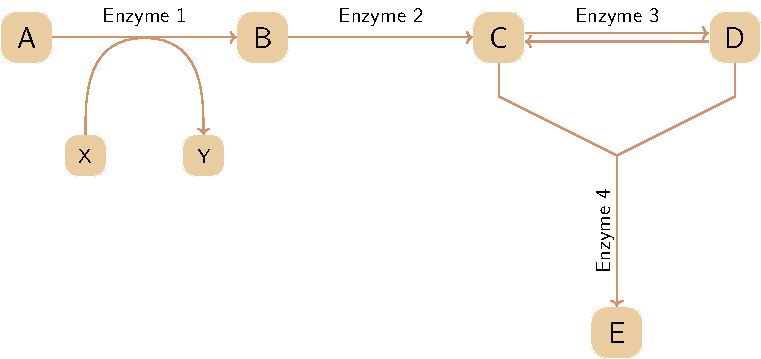
\includegraphics{images/pathway.pdf}
    \caption[Example metabolic pathway]{This figure illustrates a hypothetical metabolic pathway. Chemical reactions are catalysed by specialised proteins known as enzymes, which accelerate the rate at which metabolites are converted. The image depicts that some reactions require extra metabolites, and other produce extra chemical compounds. The pointed arrows represent the ``flow of matter'', \ie the fact that one metabolite is converted to another one, thus implicitly describing the input and output of the pathway. In this case, the inputs are the metabolites \term{A} and~\term{X}, and the outputs are the metabolites \term{E} and~\term{Y}.}
    \label{fig:pathway}
\end{figure}

While these chemical reactions usually occur within living organisms as a continuum, \ie there is no naturally defined boundary between metabolic pathways, dividing the high amount of distinct chemical reactions into manageable groups simplifies the study of metabolism. For example, the glucose produced by photosynthesis, in plants, is converted into other molecules, but even though the two processes happen simultaneously, each is described by a distinct pathway.

Knowing the components of a metabolic pathway and how they interact with one another is extremely helpful:
\begin{paralist}
    \item a metabolic pathway is a means of effective communication regarding the metabolism of various organisms~\citep{Papin2003};
    \item it enables the mathematical analysis of a complete metabolic system, since they correspond to precise mathematical descriptions of cellular properties~\citep{Papin2003}; and
    \item this information can provide insight into how organisms respond to failures in the pathway (such as the absence of an enzyme)~\citep{Baumgartner2011}.
\end{paralist}
Furthermore, inside cells, many different processes occur at the same time, with thousands of molecules being converted concurrently. As such, to quickly estimate the effect of changing something in a pathway, assistance from computerised system is required.

What makes metabolic pathways multidisciplinary is the fact that, to fully describe them, we need not just the metabolites that are converted and the molecular functions that are carried out, but also the drugs that interfere with the pathway and the diseases caused by pathway defects or other malfunctions. The Kyoto Encyclopedia of Genes and Genome (KEGG \mdash \url{http://www.genome.jp/kegg/kegg2.html}) is a collection of databases on biological systems. One of these databases is \kegg{pathway}, which categorises $269$~pathways into a hierarchy, and annotates each pathway with:
\begin{paralist}
    \item chemical compounds,
    \item enzymes,
    \item drugs that affect the pathway, and
    \item diseases that are associated with the pathway.
\end{paralist}
Annotation is done with concepts from other KEGG databases. The concepts linked to in these annotations are not from the reference ontologies mentioned in \appref{app:ontologies}, but conversion to \ontology{GO} and \ontology{CHEBI} can be performed, using KEGG's own internal tables, which map compound and drug concepts to \ontology{CHEBI}, and genes to UniProt identifiers (which can be used to find \ontology{GO} annotations for the genes). Diseases, however, have no link to reference ontologies. As such, an additional step was executed to convert KEGG diseases into Human Disease Ontology (\ontology{DOID}) identifiers.
% \appref{app:kegg-conversion} contains a detailed description of this conversion process.

\tabref{tab:pathways-summary} shows a summary of the annotations for these pathways, using the same statistics presented for the previous multi-domain dataset. Notice that in this dataset, there is not a one-to-one correspondence between domains and ontologies, since both drugs and metabolites are represented as \ontology{CHEBI} concepts. I decided to keep the two domains separate since they encode different information about the pathways.

\begin{table}
\caption[Summary of the annotation in the metabolic pathways dataset]{This dataset corresponds to $269$~pathways extracted from KEGG. Note that a domain in this dataset does not precisely correspond to an ontology, as both drug and metabolite annotations use concepts from \ontology{CHEBI}. The first two columns describe the domains and ontologies used to annotate the resources. The rest of the columns provide statistics for each domain.}
\label{tab:pathways-summary}
\centering
\small
\begin{tabular}{llrrr}
\toprule
\textbf{Domain} & \textbf{Ontology} & \textbf{Coverage} & \textbf{Volume} & \textbf{Diversity} \\
\midrule
Diseases            & \ontology{DOID}  &  79.2\% &  9.08 &  756 \\
Drugs               & \ontology{CHEBI} &  42.4\% & 30.30 & 1381 \\
\ontology{GO} terms & \ontology{GO}    & 100.0\% & 32.45 & 3210 \\
Metabolites         & \ontology{CHEBI} &  79.9\% & 21.37 & 2628 \\
\bottomrule
\end{tabular}
\end{table}

Like in the case of epidemiology resources, a database of pathways needs a multi-domain semantic similarity measure to be able to properly make use of all the information available about each pathway in order to answer user requests with the most relevant resources. Additionally, semantic similarity in metabolic pathways can also be used to
\begin{paralist}
    \item reconstruct phylogenetic trees depicting the common metabolic history of a group of organisms~\citep{Heymans2003a}, and
    \item find suitable model organisms in the study of diseases related to a certain metabolic condition~\citep{Forst1999}.
\end{paralist}
Single-ontology semantic similarity has been researched in this domain by \citet{Clemente2005}, which used similarity of proteins based on their \ontology{GO} annotations, and \citet{Grego2010}, which used instead semantic similarity between the metabolites of the pathways based on \ontology{CHEBI}.

By gathering metabolic pathway information in this way, I effectively created a dataset of pathways annotated with \ontology{CHEBI}, \ontology{GO} and \ontology{DOID} concepts, which was further used in semantic similarity studies (see \chpref{chap:multidomain}).


\section{Biochemical Models Dataset} \label{sec:data/biomodels}

A third area where multi-domain semantic similarity can be of service corresponds to models of biological systems, or biomodels, for short. This type of information is similar to the one of the previous dataset: like a metabolic pathway, a biomodel is a description of a chemical process that happens inside the cell, or within its immediate surroundings. In contrast, however, a biomodel is more computationally oriented. It represents the metabolites and enzymes involved in the reactions but also the cellular components and anatomical location where they occur, including their volume, and the equations that describe the reaction velocity with respect to the concentration of the metabolites and enzymes.

Like in the previous two scenarios, multi-domain semantic similarity is useful here as well, primarily to enable searching capabilities within a database of biomodels. Other applications include
\begin{paralist}
    \item clustering the biomodels according to similarity in order to find common patterns in different organisms, which can be used to transfer knowledge from one organism to another; and
    \item using semantic similarity to assist the act of annotating the models, by analysing similar biomodels and generating new annotation suggestions to increase the accuracy of the annotations given by an author~\citep{Schulz2012}.
\end{paralist}

The EBI Biomodels Database (\url{http://www.ebi.ac.uk/biomodels-main/}) contains formal descriptions of mathematical models of biochemical systems~\citep{Li2010a,Juty2015}. These biomodels are annotated with concepts from the relevant domains, including chemical compounds, enzymes, biological processes and anatomical entities.

% For example, the biomodel that represents the complement system~\citep{Liu2011}, a part of the immune system, includes annotations to:
% \begin{itemize}
%     \item \term{N-Acetyl-D-glucosamine} and \term{Phosphocholine} (chemical compounds);
%     \item \term{Portion of plasma} and \term{Extracellular region} (anatomical locations);
%     \item \term{Dendrite} and \term{Mitochondria} (cellular locations);
%     \item several proteins (such as \term{Uniprot:P01024}) that are responsible for performing the functions of this system and which have themselves \ontology{GO} annotations based on their functions.
% \end{itemize}

The models in this dataset are annotated with the reactions that they represent, the chemical compounds involved in the reactions (both metabolites and enzymes) and the cellular components where the reactions occur. This information is frequently (but not always) accompanied with links to ontologies such as \ontology{GO} and \ontology{CHEBI}. For example, reactions are linked to concepts from \ontology{GO}; chemical compounds are linked to \ontology{CHEBI} concepts, \kegg{compound} terms, and InterPro and UniProt identifiers; protein complexes that participate in the reaction and cellular components are linked to the Cellular Component branch of \ontology{GO} (which represents complexes as well as membrane-delimited components); cell components are also linked to \ontology{FMA} concepts; and physical quantities, like mass and electric charge, are linked to \ontology{PATO} concepts.

Given the complexity of these annotations, I decided to make some conversions and ignore some annotations. For example, I ignored \kegg{protein} terms (there are only~$3$ in the whole set of annotations). \kegg{compound} terms were converted to \ontology{CHEBI} concepts when possible (compounds without a correspondence were ignored as well), and UniProt and InterPro identifiers were converted into the \ontology{GO} annotations for those proteins. This resulted in each model having annotations to \ontology{CHEBI}, \ontology{FMA}, \ontology{GO} and \ontology{PATO}. A summary of the annotations for the biomodels is given in \tabref{tab:biomodels-summary}.

\begin{table}
\caption[Summary of the annotation in the biomodels database]{This dataset corresponds to the $282$~distinct biomodels extracted from the BioModels website. The first column describes the ontologies used to annotate the resources. The rest of the columns provide statistics for each ontology.}
\label{tab:biomodels-summary}
\centering
\small
\begin{tabular}{lrrr}
\toprule
\textbf{Ontology} & \textbf{Coverage} & \textbf{Volume} & \textbf{Diversity} \\
\midrule
\ontology{CHEBI} & 55.0\% &  6.99 &  261 \\
\ontology{FMA}   &  3.9\% &  1.18 &   11 \\
\ontology{GO}    & 90.8\% & 55.43 & 3314 \\
\ontology{PATO}  & 95.4\% &  1.06 &    5 \\
\bottomrule
\end{tabular}
\end{table}

I extracted from this dataset $250$~pairs of biomodels (for a total of $282$~distinct biomodels), with the aim of having a Systems Biology expert assess the degree of similarity between each pair. The data in this \emph{gold-standard} corresponds to the models and their annotations from the corresponding ontologies. To ensure a good coverage of all similarity values, $100$~pairs were generated randomly and the other~$150$ were generated based on a preliminary semantic similarity calculation, in order to have a balanced distribution of similarity values. To this effect, I first calculated semantic similarity on all the biomodel pairs and divided the pairs into three categories: one for similarity values below~$0.33$, another for values between $0.34$ and~$0.67$, and another for values higher than~$0.67$. This ensured that pairs covering the full range of similarity were included in the gold-standard. The $100$~random pairs were generated to cover the possibility that the preliminary similarity values were not significant.

The $250$~pairs were classified by the expert as ``not similar'', ``somehow similar'', ``similar'', and ``very similar''. Expert assessment was conducted based on a web-tool that I designed for that effect. \figref{fig:biomd} displays some screen-shots of the tool.

\begin{figure}
    \centering
    \subbottom[The main page of the similarity assessment tool%
               \label{fig:biomd/page}]{%
        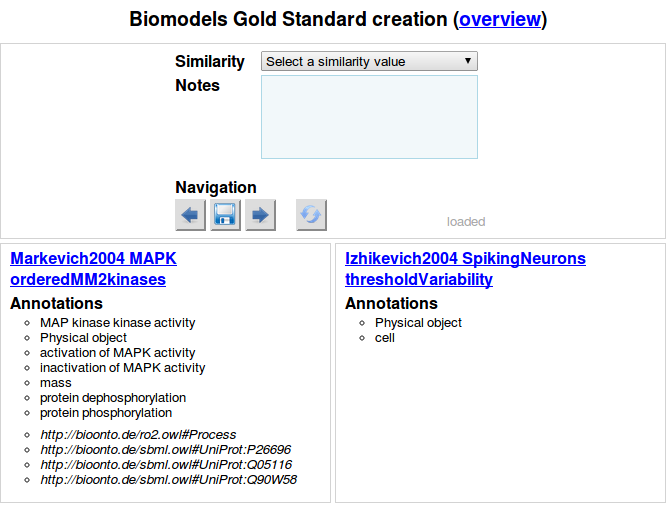
\includegraphics[scale=0.55]{images/biomd-page-2.png}%
    }
    \vspace{\baselineskip}
    \subbottom[A detail of the similarity selection section%
               \label{fig:biomd/detail}]{%
        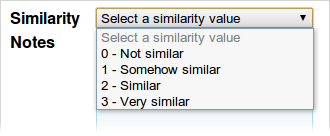
\includegraphics[scale=0.55]{images/biomd-detail.png}%
    }
  
    \caption[The EBI Biomodels similarity assessment tool]%
    {\subcaptionref*{fig:biomd/page} Each model is accompanied with the set of ontology concepts that annotate it. In the bottom of this panel, there are control buttons to navigate through the $250$~pairs and a ``Notes'' section to allow the expert to make their own notes, for future reference. \subcaptionref*{fig:biomd/detail} The similarity value can be chosen between $0$ and~$3$.}
    \label{fig:biomd}
\end{figure}
